\chapter{Supplementary material}

%\resp{Franco Aquistapace Tagua}
% TASK 6
\section{Song-Havlin-Makse self-similar model}
\label{sec:SHM_SM}
 
\subsubsection*{Algorithmic implementation of the renormalisation procedure}
The renormalisation of a given network is performed algorithmically as follows:

\begin{enumerate}
	\item Initialise a box with a randomly picked node.
	\item For every remaining node $i$, add it to the box if $\max_{j\in B} d(i,j) \leq L_B$, where $B$ contains the nodes currently in the box, and $d(i,j)$ is the shortest path between nodes $i$ and $j$.
	\item Repeat steps 1. and 2. with the remaining available nodes until all nodes are assigned to a box.
\end{enumerate}

\subsubsection*{Correlation profiles}

The correlation profile $R(k_1, k_2) = P(k_1, k_2) / P_r(k_1, k_2)$ is defined as the ratio between the joint degree--degree probability distribution of the network of interest, $P(k_1, k_2)$, and the joint degree--degree probability distribution of a randomised uncorrelated version of the same network, $P_r(k_1, k_2)$, where the links have been randomly rewired while preserving the degree distribution. 

In this work, the joint degree--degree probability distribution is estimated in a frequentist approach, by considering all equivalent instances as observations. For example, to obtain $P(k_1, k_2)$ for the minimal model graph with $e=1.0$, the degree--degree pairs of the 10 graphs generated for $e=1.0$ are collected. Then, the joint probability for a given pair $(k_1, k_2)$ is calculated as in Eq. \ref{eq:P_joint_task_6_SM}:

\begin{equation}
	P(k_1, k_2) = \frac{N_{obs}(k_1, k_2)}{N_{obs, tot}} \ \ ,
	\label{eq:P_joint_task_6_SM}
\end{equation}
where $N_{obs}(k_1, k_2)$ is the number of occurrences of the pair $(k_1, k_2)$, and $N_{obs, tot}$ is the total number of observations. The same methodology is applied for the calculation of $P_r(k_1, k_2)$. No interpolation is done for pairs $(k_1', k_2')$ that are not observed, and their probability is thus taken as $P(k_1', k_2') = 0$.


\subsubsection*{Scaling relations}

The descriptor $N_B(L_B) / N$ is defined as the ratio between the number of original nodes, $N$, and the number of boxes, $N_B$, obtained after performing a renormalisation step with box size $L_B$. Meanwhile, the descriptor $\mathcal{S}(L_B) = k_B(L_B) / k_{hub}$ is the ratio between the maximum degree of the boxes after a renormalisation step with box size $L_B$, $k_B(L_B)$, and the maximum degree of the among the original nodes, $k_{hub}$. For both scaling relations, $N_B(L_B) / N$ and $\mathcal{S}(L_B)$, the mean value and standard deviation is obtained for each $L_B$ from the 10 networks generated for both cases $e=1.0, 0.8$. From the obtained results, the theoretical models proposed in the source material \cite{song2006origins} are fitted. 

For the fractal case $e=0.8$, $N_B(L_B) / N$ and $\mathcal{S}(L_B)$ are described, respectively, by Eqs. \ref{eq:N_fractal_SM} and \ref{eq:S_fractal_SM}:

\begin{equation}
	N_B(L_B) / N = C_N (L_B + L_0)^{-d_B}
	\label{eq:N_fractal_SM}
\end{equation}

\begin{equation}
	\mathcal{S}(L_B) = C_S (L_B + L_0)^{-d_k}
	\label{eq:S_fractal_SM}
\end{equation}
where $L_0$, $d_B$, $d_k$, $C_N$ and $C_S$ are parameters fitted from the data. The data points with $L_B < 8$ were excluded from the fit of $N_B(L_B) / N$, and those with $L_B < 12$ were excluded from the fit of $\mathcal{S}(L_B)$. From the fit, the values $d_B = 2.83$ and $d_k = 2.91$ are obtained. 

On the other hand, for the non--fractal case $e=1.0$, $N_B(L_B) / N$ and $\mathcal{S}(L_B)$ are described, respectively, by Eqs. \ref{eq:N_non_fractal_SM} and \ref{eq:S_non_fractal_SM}:

\begin{equation}
	N_B(L_B) / N = C_N \exp(-L_B / L_0)
	\label{eq:N_non_fractal_SM}
\end{equation}

\begin{equation}
	\mathcal{S}(L_B) = C_S \exp(-L_B / L_0)
	\label{eq:S_non_fractal_SM}
\end{equation}
where again $L_0$, $C_N$ and $C_S$ are fitted from the data. In this case, the data points with $L_B > 12$ are excluded from the fit of both $N_B(L_B) / N$ and $\mathcal{S}(L_B)$.



% TASK 15
\section{Sandpile dynamics on complex networks}
\label{sec:SOC_SM}

\subsubsection*{Bak-Tang-Wiesenfeld sandpile model simulations}

In general, for each avalanche event in the Bak-Tang-Wiesenfeld model simulations, the following quantities are registered:
\begin{itemize}
	\item Avalanche area $A$: defined as the number of distinct nodes participating in an avalanche event.
	\item Avalanche size $S$: defined as the number of toppling events in a given avalanche.
	\item Number of toppled grains, $G$.
	\item Duration of the avalanche, $T$.
\end{itemize}

For the simulations on interdependent networks the following observations are additionally registered: subgraph where an avalanche originates, local size of the avalanche in the origin subgraph and inflicted size of the avalanche on the non-origin subgraph.

\subsubsection*{Generation of scale--free networks}

In this work, the static model from \cite{goh2003sandpile} is used to generate scale--free networks with desired properties as follows: 

Here, the networks are generated with $2\times10^5$ nodes, average degree $\langle k\rangle=4$ and degree exponents $\gamma\in(2,\infty)$.

Isolated nodes and possibly other small subgraphs are removed from the system by only keeping the largest connected component. In general, the amount of removed nodes is not significant when compared to the size of the remaining network.

\subsubsection*{Characteristics of avalanches in scale--free networks}


\begin{figure}[!h]
	\begin{center}
	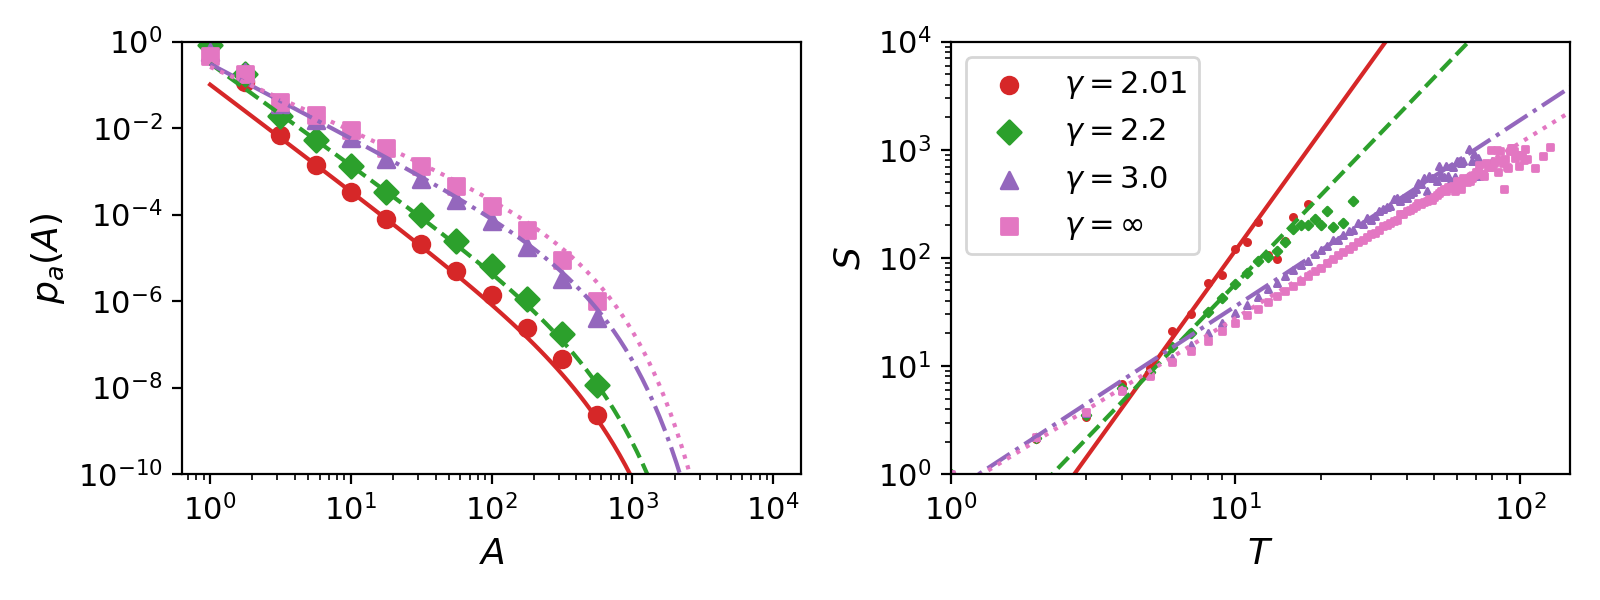
\includegraphics[scale=0.75]{./images/task_15/SM_scale_free_distributions.png} 
	\end{center}
	\caption{Caption. \\} 
	\label{fig:SM_scale_free_distributions} 
\end{figure}


\subsubsection*{Generation of interdependent regular networks}

In this work, each interconnected network is first initialised as two separate $z$-regular subgraphs, $G_A$ and $G_B$, with uniform degree $z=3$ and $2\times10^3$ nodes each. Then, the connection between these subgraphs is done by means of uncorrelated Bernoulli coupling, as follows: for each node in $G_A$ a random number is uniformly sampled from $(0,1)$, if that number is smaller than a threshold $p$ then an available node from $G_B$ is uniformly sampled and a link to it is established. The selected node from $G_B$ is then removed from the set of available nodes, so that each node in $G_A$ can be connected at most to a single node from $G_B$, and vice versa. 


\subsubsection*{Characteristics of avalanches in interdependent networks}

\begin{figure}[!h]
	\begin{center}
	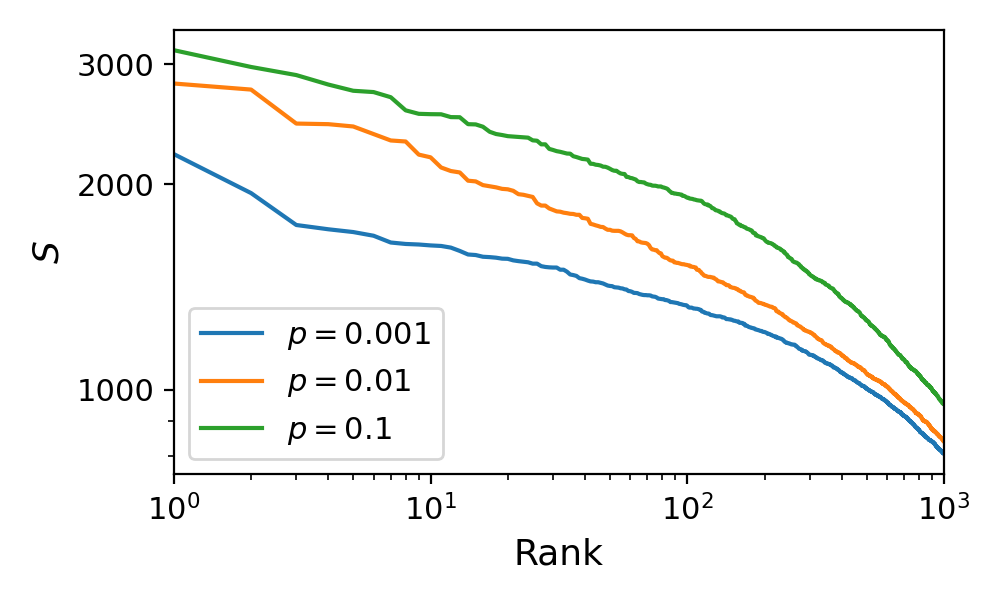
\includegraphics[scale=0.75]{./images/task_15/SM_large_avalanche_rank_plot_joint_AB.png} 
	\end{center}
	\caption{Caption. \\} 
	\label{fig:SM_large_avalanche_rank_plot_joint_AB} 
\end{figure}



\newpage